%!TEX root = ../dokumentation.tex

\chapter{Implementierung des Tools}

\section{Grundstruktur der Applikation}

Die Grundstruktur der Applikation basiert auf zwei im MATLAB App Designer erstellten Applikationen. Der Hauptapplikation, welche das Aufrufen einzelner Funktionalität ermöglicht, sowie den Graphen der erstellen Visualisierungen darstellt, und die Applikation zur Konfiguration der Samples, welche parallel zur Hauptapplikation als Pop-Up geöffnet werden kann, jedoch nicht ohne diese verwendbar ist. Als dritte Struktur wurde die sogenannte WithSamplesParser-Klasse erstellt, welche alle Funktionalitäten bezüglich der Messdatenverarbeitung und Darstellung enthält. Dazu gehören das Einlesend und Umstrukturieren der Messdaten auf ein passendes Format, sowie das Erstellen eines Graphen mit der passenden Konfiguration. Diese Funktionen werden dabei ebenfalls aus der Hauptapplikationen gestartet und benötigen diese deshalb auch als Grundlage.

\begin{figure}[!htbp]
	\centering
	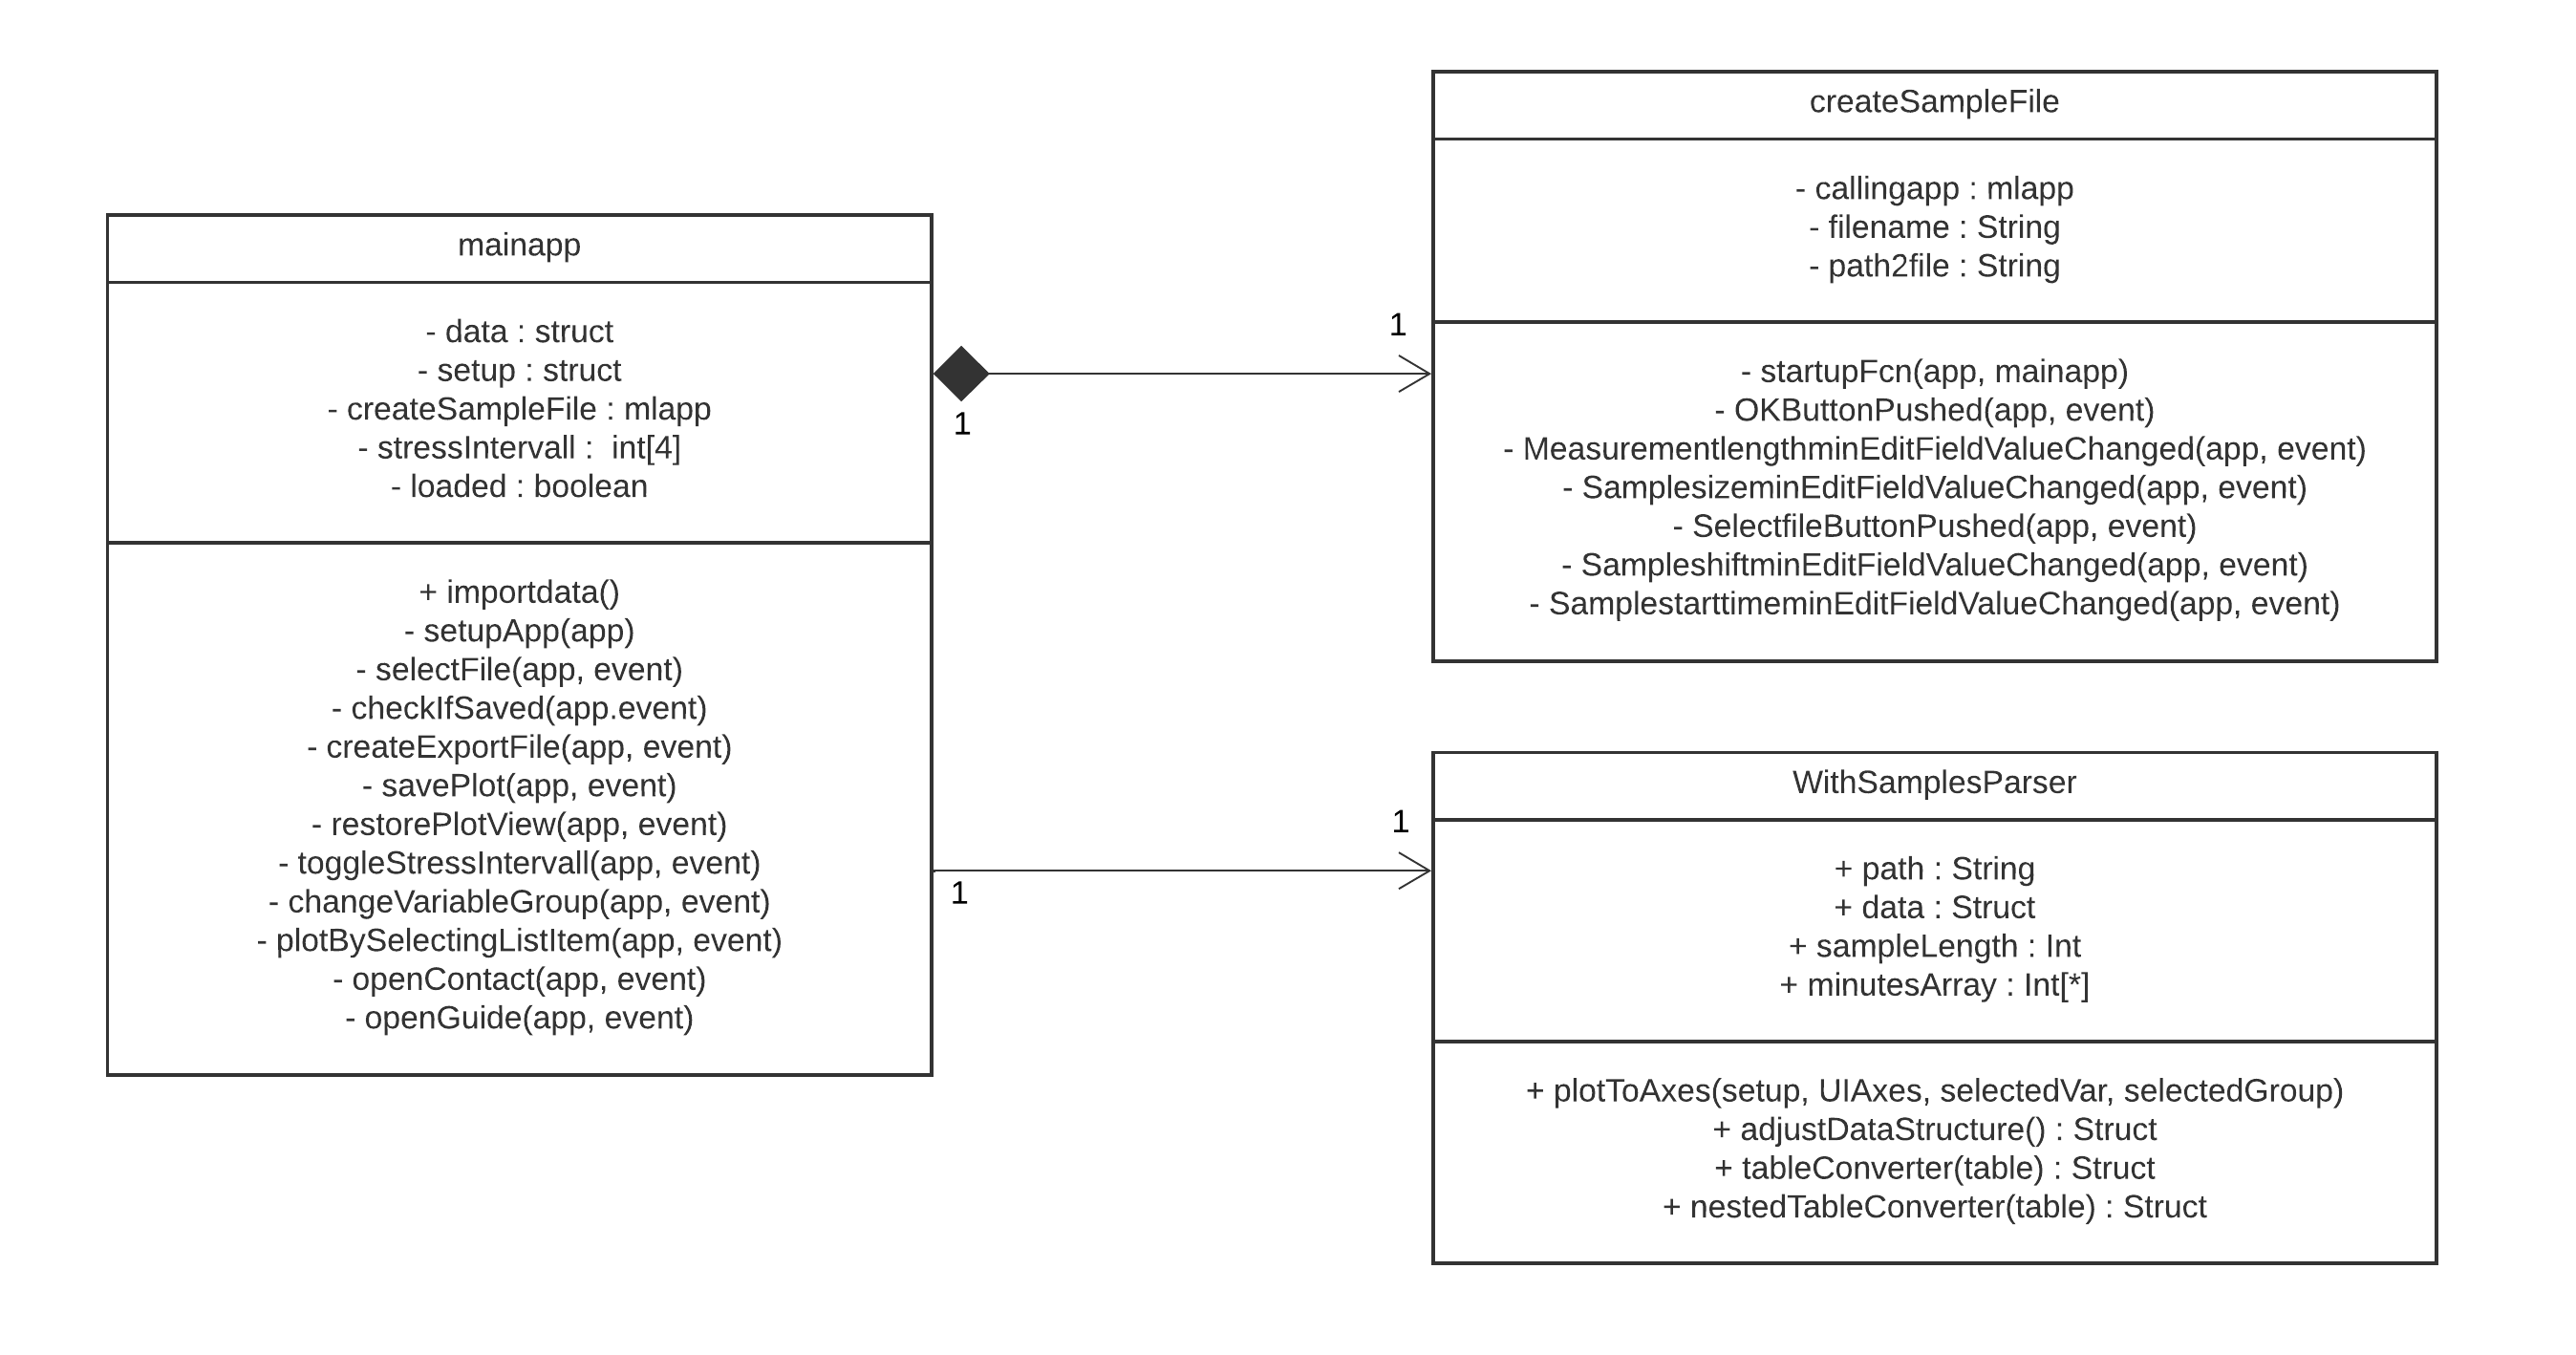
\includegraphics[width=1\linewidth]{klassendiagramm}
	\caption{Klassendiagramm der fertigen Applikation}
	\label{fig:klassendiagramm}
\end{figure}

\subsection{Layout und Komponenten}

Der MATLAB App Designer setzt bei der Erstellung von Applikation auf Code-Generierung. Der App Designer ist eine eigenständige MATLAB Applikation, welcher über eine Auswahl bereits vorgefertigter Komponenten, wie verschiedene beispielsweise Buttons, Container oder Eingabefelder verfügt. Um eine Applikation zu erstellen, können diese einfach beliebig kombiniert und visuell angepasst werden. Aus den verwendeten Komponenten wird dann eine Klasse generiert, welche beim Ausführen instanziiert wird. Diese Klasse enthält einen genauen \glqq Bauplan\grqq{} der späteren Applikation. Funktionen, welche beispielsweise durch das Klicken eines Buttons ausgelöst werden basieren auf sogenannten \textbf{Callbacks} (siehe Setup der Applikation). Diese werden direkt als Methoden der App-Klasse definiert und können nicht generiert werden. Jede Komponente kann mehrere dieser Callbacks besitzen.

\lstinputlisting[language=Matlab,numbers=left,firstline=1,lastline=8,caption={Auszug einiger verwendeter App-Komponenten}]{code/appComponents.m}

Die Grundstruktur der implementierten Applikation bildet die \textbf{Figure-Komponente}. Diese legt die Fenstergröße fest und ist die Grundlage der Applikation in der die einzelnen Unterkomponenten eingefügt werden. Um eine gewisse Grundstruktur in das Aussehen zu integrieren wird ein \textbf{Grid-Layout} nächste Stufe der Komponenten-Hierarchie eingebaut. Dies ermöglicht das korrekte Positionieren der einzelnen Komponenten innerhalb der Applikation und damit auch die symmetrische Konsistenz von Rahmen- und Komponentenabständen, welche im grundlegenden Design-Konzept definiert wurden. Außerdem fügt es der Applikation eine umfassende Responsiveness hinzu, wodurch das Verwenden der Applikation in unterschiedlichen Monitorgrößen und Fenstergrößen ermöglicht werden kann ohne ungewollte Nebeneffekte herbeizuführen.

\todo{Die Applikation besteht aus den folgenden Elementen... (UIAxes, ListBox, etc.)}


\todo{Bild der fertigen Applikation}

\section{Setup der Applikation}

Die Export-Daten von Kubios haben ein Problem in der Konsistenz ihrer Datensätze. So sind innerhalb der MAT-Datei lediglich reine Zahlenwerte und die spezifischen Identifier der Parameter zu finden. Es fehlen wichtige Elemente wie beispielsweise ein genauer Name und die Einheit der Parameter. Um nun die Visualisierungen einzelner Parameter mit allen wichtigen Informationen versorgen zu können, muss eine entsprechende Mapping-Datenbank vorhanden sein, welche manuell konfiguriert werden muss.

Die Applikation lädt sich hierzu beim Starten eine entsprechende MAT-Datei als Variable in den Workspace. Diese Datei enthält die Mappings der einzelnen Parameter sortiert nach ihrer jeweiligen Gruppierung. So ergeben sich drei Setupstrukturen im Tabellenformat mit den Spalten Index, Kurzbezeichner, Kurzbeschreibung, Einheit und Gruppierung. Mit Hilfe des von Kubios erzeugten Index lassen sich nun alle dazugehörigen Informationen aufrufen und verwerten. Zudem wird diese Setup-Datei verwendet um zu Beginn alle vorhandenen Parameter unter ihrer jeweiligen Gruppierung zur ListBox-Komponente hinzuzufügen, sodass der Nutzer später diese Auswählen kann.

Zusätzlich wurde eine Helper-Funktion geschrieben, welche es ermöglicht aus einer Excel-Datei das Setup zu generieren, um die Handhabung bzw. Veränderung des Mappings zu ermöglichen. Dazu können einfach neue Elemente in die Tabelle mit aufgenommen oder bereits bestehende Einträge verändert bzw. gelöscht. Diese Funktion ist jedoch der Entwicklung vorenthalten, da das Verändern bestehender Workspace-Variable nach der Installation oder während des Betriebs der Applikation nicht passend umsetzbar ist. 

\begin{figure}[H]
	\centering
	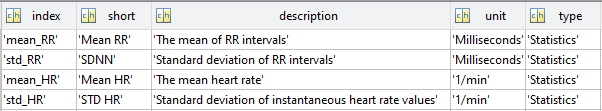
\includegraphics[width=1\linewidth]{setupStruktur}
	\caption{Auszug aus der Struktur der Setup-Datei}
	\label{fig:setupStruktur}
\end{figure}


\section{Erstellung der Samples}

\todo{Wim schreibt was er gemacht hat :)}
\todo{Die Applikation besteht aus den folgenden Elementen... (UIAxes, ListBox, etc.)}

\section{Visualisierung der Daten}

Im folgenden Teil der Implementierung sollen die einzelnen Schritte und Funktionen dargestellt werden, welche zum schlussendlichen Visualisieren und Auswerten der Daten beitragen. Dazu gehören die Verarbeitung der Daten und die Datenstruktur im Backend der Applikation, sowie das Darstellen des Graphen mit Hilfe der Plot-Funktion und die dazugehörigen erweiternden Funktionen wie beispielsweise das Hervorheben des Belastungsintervalls.

\subsection{Datenstruktur und Datenverarbeitung}

Um das schnelle Visualisieren und Verarbeiten der Daten muss eine zentrale Datenstruktur entwickelt werden, die hohe Übersichtlichkeit, gute Erweiterbarkeit, sowie möglichst minimalistisch und kompakt aufgebaut ist. Zudem ist es wichtig ein passendes Format für die Visualisierungsfunktionen von MATLAB zu verwenden, da diese nur bestimmte Datenformate als Eingabe-Parameter akzeptiert. Die Rohdaten sind dabei sehr verschachtelt und es sind lange Zugriffsketten nötig, um an die korrekte Datenwerte zu gelangen. Außerdem fehlt es oft an Konsistenz. Während ein Großteil der Parameter als Tabelle vorliegt und mittels der passenden Spalte ausgelesen werden können, sind einige in eine weitere Struktur verschachtelt oder es liegen Parameter in einer Liste unter einem allgemeinen Bezeichner vor und müssen mit dem passenden Index extrahiert werden. Deshalb benötigen die eingelesene Daten eine vorläufige Anpassung bevor sie visualisiert werden können. Aus diesem Grund muss das eingelesene MAT-File angepasst werden, um nicht für jeden Parameter eine separate Zugriffsfunktion implementieren zu müssen.

\begin{figure}[H]
	\centering
	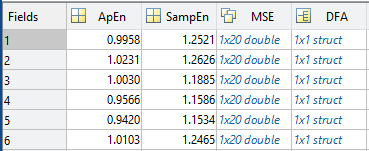
\includegraphics[width=0.7\linewidth]{rawData}
	\caption{Verschachtelungsprobleme der unverarbeiteten Export-Daten}
	\label{fig:rawData}
\end{figure}

% Quelle für Key-Value/Dictionary Python
Das Einlesen des MAT-Files erfolgt über den Menüpunkt \glqq Load measurement\grqq{}. Dieser öffnet das Dateisystem des Betriebssystems und ermöglicht das Auswählen einer Datei. Gleichzeitig wird ein Objekt der Parser-Klasse \textbf{WithSampleParser} instanziiert, welche die Inhalte der Datei speichert und eine konsistente Datenstruktur anlegt.\\
Als Grundkonzept wird dazu ein Struct angelegt. Dieses lässt sich mit einem Python-Dictionary vergleichen, in dem die Elemente mittels Key-Value-Paaren abgespeichert sind. Ein Datensatz lässt sich dann einfach mit Hilfe des entsprechenden Keys aufrufen. Zusätzlich ist es möglich dieses zu verschachteln und unter einem Key ein weiteres Key-Value-Paar zu speichern. So lässt sich eine hierarchische Beziehung zwischen den unterschiedlichen Parametern und Datensätzen erzeugen.

Das erzeugte Struct besteht aus vier Ebenen. Auf obersten Ebene sind die Gruppierungen der Parametern zu finden. Für die Parameter der Herzmessdaten wurden hier die bereits von Kubios HRV Premium vordefinierten Gruppierungen Time-Domain, Nonlinear sowie Frequency-Domain im Zeit- und Frequenzbereich verwendet. Unterhalb dieser Bezeichner befinden sich dann alle zugehörigen Parameter. Im Falle der Frequency-Domain wird hier noch die Ebene der Darstellung, also Zeit- oder Frequenzbereich, eingeschoben, da hier die Parameter-Bezeichner identisch sind und so eine Unterscheidung unmöglich wäre. Auf tiefster Ebene ist dann jedem Parameter ein Datensatz als Liste mit genauen Werten zugeordnet. Ein Eintrag in der Liste entspricht dabei immer dem Mittelwert des Parameters für den Zeitraum der zuvor konfigurierten und exportierten Samples. Diese Liste bildet eine gute Grundlage für die Visualisierung der Daten mit Hilfe der vorhandenen MATLAB-Funktionen. Außerdem ist es möglich diese für gegebene Anforderungen zu manipulieren.

\begin{figure}[H]
	\centering
	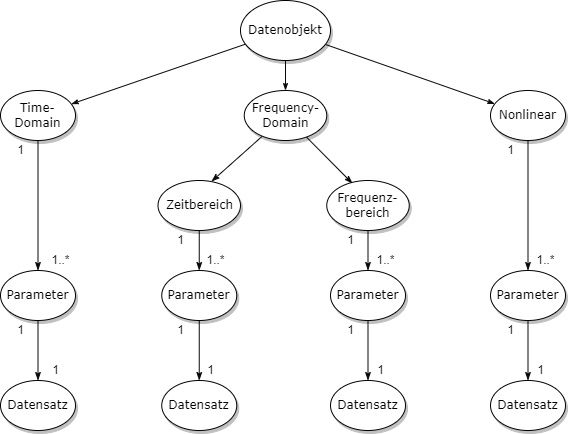
\includegraphics[width=0.8\linewidth]{datenstruktur}
	\caption{Baumstruktur zur Veranschaulichung der Datenstruktur}
	\label{fig:datenstruktur}
\end{figure}

Um diese Struktur bilden zu können werden einige Funktionen zur Anpassungen durchlaufen. Zuerst wird die Tabelle invertiert. Das lässt sich darauf zurückführen, dass ein Großteil der Daten innerhalb einer Spalte gespeichert und der Zugriff beim Visualisieren der Daten mit Hilfe der MATLAB-Funktion auf als Reihe gespeicherte Daten präferiert wird. Hierzu wurde eine Methode implementiert, welche alle Spalten und die Parameter-Bezeichner einliest, invertiert und als Struct abspeichert.

\lstinputlisting[language=Matlab,numbers=left,firstline=1,lastline=10,caption={Konvertieren einer MATLAB Tabelle in ein Struct}]{code/tableConverter.m}

Für das Extrahieren von verschachtelten Parametern innerhalb der Tabelle müssen zusätzliche Schritte ausgeführt werden. Hierbei muss die Struktur, welche anstatt eines direkten Wertes vorliegt, aufgelöst werden. Im ersten Schritt werden dabei alle unwichtigen Parameter, die keinen Sample-Bezug besitzen gelöscht. In einer Schleifen werden dann alle restlichen Parameter kopiert und zu den restlichen Einträgen des zuvor erstellten Structs hinzugefügt. Somit ist die Verschachtelung von zwei Ebenen auf eine reduziert.

\lstinputlisting[language=Matlab,numbers=left,firstline=1,lastline=9,caption={Auflösen verschachtelter MATLAB Tabellen in ein Struct}]{code/nestedTableConverter.m}

Um eine Reduzierung mehrerer Parameter auf einen allgemeinen Bezeichner rückgängig zu machen wurde folgendes Vorgehen implementiert. Innerhalb des Datensatzes handelt es sich hier um den Parameter \glqq Multiscale entropy\grqq{}, welcher zwanzig unterschiedliche Skalierungsfaktoren besitzt. Diese sind innerhalb eines Bezeichners als Liste aus zwanzig Werten angelegt. Für die korrekte Visualisierung müssen diese jedoch als einzelne Parameter der Struktur angeziegt werden, wobei der Datenwert an der ersten Stelle der Liste dem Wert für den Skalierungsfaktor eins entspricht. Die Auflösung erfolgt mittels zweier Iterationen. Zuerst werden alle Listen aneinander gehängt, sodass eine Matrix der einzelnen Werte entsteht. Mittels der zweiten Iteration wird diese Matrix in die einzelnen Structs aufgeteilt und der allgemeine Bezeichner mit dem Schleifen-Index als Key gesetzt.

\lstinputlisting[language=Matlab,numbers=left,firstline=1,lastline=9,caption={Auflösen eines Parameters in einer Liste anhand des Beispiel-Parameters MSE}]{code/listConverter.m}

Zum Schluss muss noch beachtet werden, dass die grundlegenden Daten keine direkten x-Werte, also exakte Zeitpunkte der Parameter-Messung, enthalten. So kann ein Datensatz lediglich mit seiner Stelle in der Liste, also für den ersten Wert x=0, zweiter Wert x=1, usw. verknüpft und visualisiert werden. Da die einzelnen Daten aber die Mittelwerte einzelner Samples sind und deren Länge im Normalfall größer einer Minute sind, muss hier ein passender Eintrag in der Datenstruktur hinzugefügt werden, um das Zuordnen der Messeinträge mit der relativen Messzeit zu ermöglichen. Hierzu wird beim Einlesen der Daten die Sample-Länge mit Hilfe der vorhandenen Informationen in der Messdatei berechnet. Dazu wird zuerst die Messzeit in Minuten umgerechnet und durch die Anzahl der Einträge, also Messwerte pro Parameter, geteilt. Da die Sample-Länge meist aber kein Teiler der Messzeit ist und es somit oft zu einem unvollständigen Sample am Ende der Messung kommt, wird die berechnete Sample-Länge noch abgerundet. Man erhält so eine genaue Minutenzahl. Hieraus lässt sich nun auch eine Liste beginnend mit der Sample-Länge erstellen, deren Schrittweite ebenfalls einer Sample-Länge entspricht. Dieser wird an das fertige Daten-Struct angehängt und als Werte für die x-Achse verwendet.

\lstinputlisting[language=Matlab,numbers=left,firstline=1,lastline=4,caption={Ermittlung von Sample-Länge und Erstellung der x-Werte}]{code/sampleLength.m}

\subsection{Plot-Funktion}

Die Hauptaufgaben der Plot-Funktion (dt. graphisch darstellen) sind das Auswählen des richtigen Datensatzes anhand einer gegebenen Gruppe und dem zugehörigen Messparameter, sowie das Verknüpfen der Daten mit dem Koordinatensystem und das Anpassung der Koordinatenachsen auf den passenden Stand.

Die Plot-Funktion wird dabei durch das Auswählen eines Messparameters in der Liste aller konfigurierten Parameter aufgerufen. Als Methode der Parser-Klasse \textbf{WithSampleParser} hat sie direkten Zugriff auf die eingelesenen Messdaten. Sie erhält dabei die setup-Konfiguration, das Koordinatensystem als UIAxes-Objekt des App Designers, den ausgewählten Parameter und dessen Gruppe. Zu Beginn wird anhand der übergebenen Gruppe, der Link auf die passende Setupstruktur und die Tabelle in der Datenstruktur ermittelt.

\lstinputlisting[language=Matlab,numbers=left,firstline=1,lastline=4,caption={Beispiel der Link-Zuordnung für Parameter-Gruppe}]{code/getGroupPlot.m}

Mit den beiden Links wird nun nach dem speziellen Parameter gefiltert und dessen Index innerhalb der Tabelle zurückgegeben. Hiermit lassen sich nun das Daten-Array, der vollständige Bezeichner, die Kurzbeschreibung und die Einheit des Parameters bestimmen. 

\lstinputlisting[language=Matlab,numbers=left,firstline=1,lastline=8,caption={Index des Parameters und dazugehörige Informationen filtern}]{code/getIndexPlot.m}

Das Daten-Array wird nun als Liste der y-Werte dem Koordinatensystem übergeben und dort als Datensatz hinterlegt. Die passenden Werte der x-Achse wurden bereits innerhalb des Einlesevorgangs der Messdaten ermittelt und repräsentieren die Länge der Messung als relative Minutenangabe. Diese werden ebenfalls mit an das Koordinatensystem angehängt. Mit Hilfe der MATLAB-eigenene Scatter-Funktion wird dem UIAxes-Objekt die Information übertragen, dass es sich um einen Scatter-Plot (dt. Streu-Graphen) handelt und die x- und y-Werte-Paare als Punkte ohne verbindende Linie dargestellt werden sollen. Hier können ebenfalls Konfigurationen für die Darstellung der Daten-Tupel im Graphen übergeben werden.

\lstinputlisting[language=Matlab,numbers=left,firstline=1,lastline=4,caption={MATLAB Scatter-Funktion}]{code/plotFunktion.m}

Im letzten Schritt wird das Aussehen des Koordinatensystems angepasst, so dass es die wichtigen Informationen wie Achsenbeschriftungen aber auch Titel und Kurzbeschreibung enthält und der Bildausschnitt angenehm für den Ersteindruck ist.

\subsection{Zusätzliche Funktionen}

\todo{Belastungsintervall, Plot speichern, Plot Restoren}